%!TEX root = ../paper.tex

% General
	%Small difference between two estimators
	In \cref{s:results:multipleGaussian} we observed that the differences in performance between the two estimators are small. 

	% Ferdosi 2 and Baakman 2
	Plotting the \mbe density as a function of the \sambe density for dataset \ferdosiTwo and \baakmanTwo, see \cref{fig:discussion:multisphere:two:mbevssambe}, we find that \sambe generally estimates densities to be higher, and nearer to the true density, than \mbe. To investigate the cause of this effect we created \cref{fig:discussion:multisphere:two:mbeLoweError} in which the point on which the absolute error of the \mbe was lower than the absolute error of the \sambe are emphasized. This plot shows that the shape-adaptive estimator outperforms the symmetric estimator on the boundary of both datasets, however the symmetric estimators seem to perform better on the center of the dataset where most points are located. It should be noted that counting the points in the center of the datasets were one estimators outperforms the other shows that the density of only approximately half of the are better estimated by the symmetric kernel. Neither dataset shows a correlation between the distance to the mean, the error and the used estimator. 

	\begin{figure}
		\centering
		\begin{subfigure}{0.23\textwidth}
			\centering
			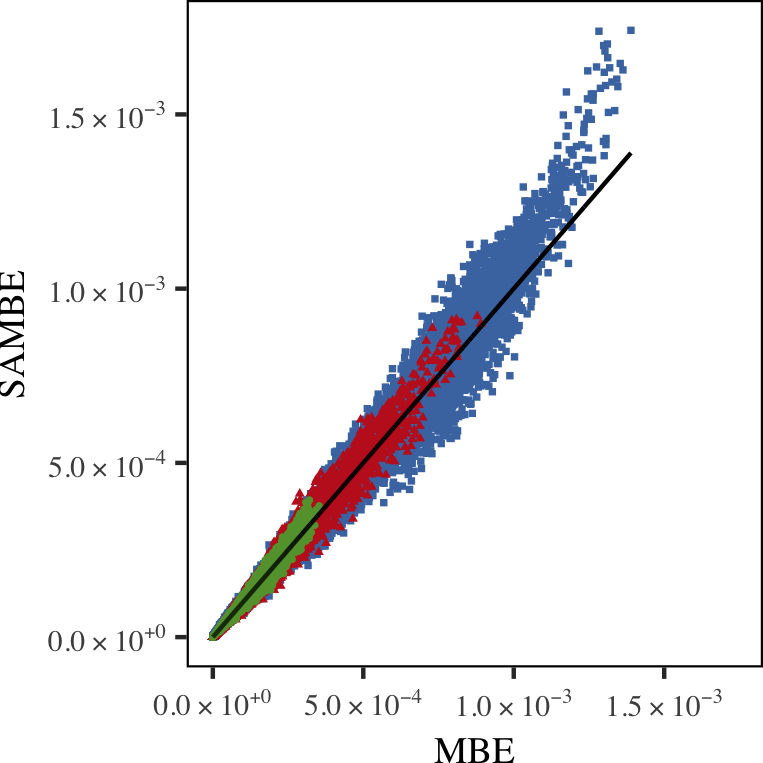
\includegraphics[keepaspectratio=true, width=\textwidth, height=0.23\textheight]{discussion/img/ferdosi_2_60000_mbe_sambe.png}
			\caption{Dataset \ferdosiTwo}
			\label{fig:discussion:multisphere:mbevssambe:ferdosi2}
		\end{subfigure}
		\begin{subfigure}{0.23\textwidth}
			\centering
			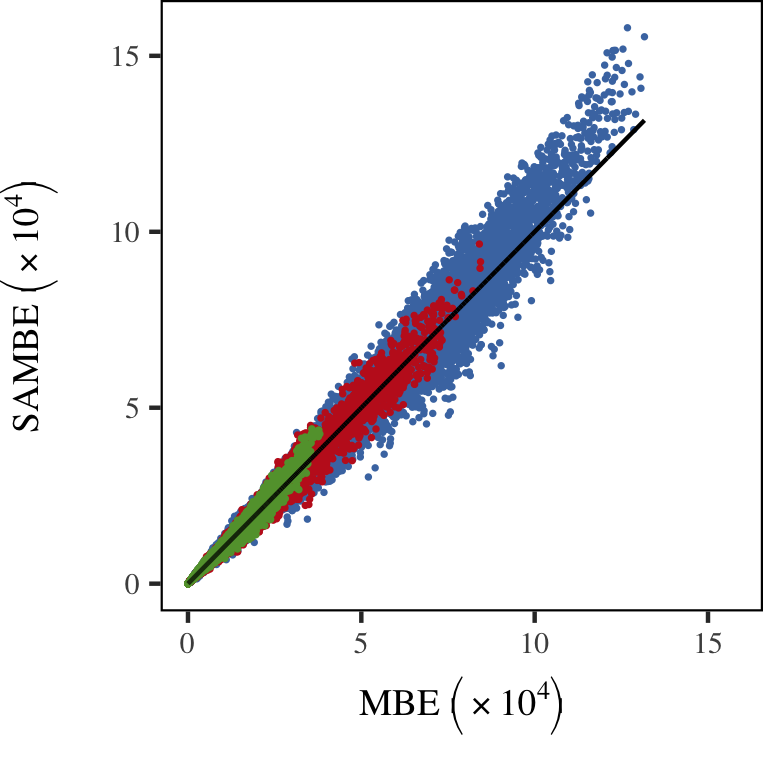
\includegraphics[keepaspectratio=true, width=\textwidth, height=0.23\textheight]{discussion/img/baakman_2_60000_mbe_sambe.png}
			\caption{Dataset \baakmanTwo}
			\label{fig:discussion:multisphere:mbevssambe:baakman2}
		\end{subfigure}	
		\caption{Plots of the density estimated by \sambe as a function of those estimated by \mbe for dataset %
			\subref{fig:discussion:multisphere:mbevssambe:ferdosi2} % 
			\ferdosiTwo and %
			\subref{fig:discussion:multisphere:mbevssambe:baakman2} %
			\baakmanTwo.
		}
		\label{fig:discussion:multisphere:two:mbevssambe}
	\end{figure}

	\begin{figure}
		\centering
		\begin{subfigure}{0.23\textwidth}
			\centering
			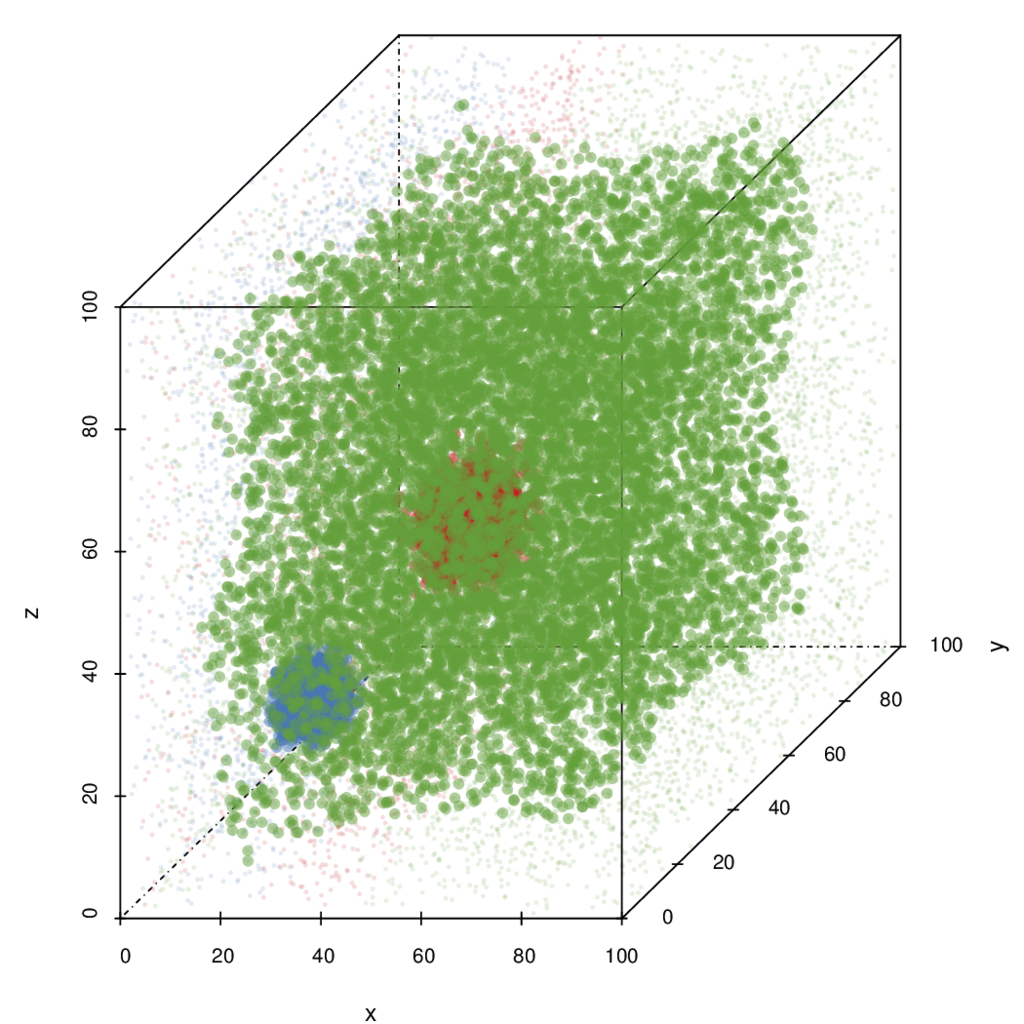
\includegraphics[keepaspectratio=true, width=\textwidth, height=0.23\textheight]{discussion/img/ferdosi_2_abs_error_mbeSmallerThansambe.pdf}
			\caption{Dataset \ferdosiTwo}
			\label{fig:discussion:multisphere:mbeLowerError:ferdosi2}
		\end{subfigure}
		\begin{subfigure}{0.23\textwidth}
			\centering
			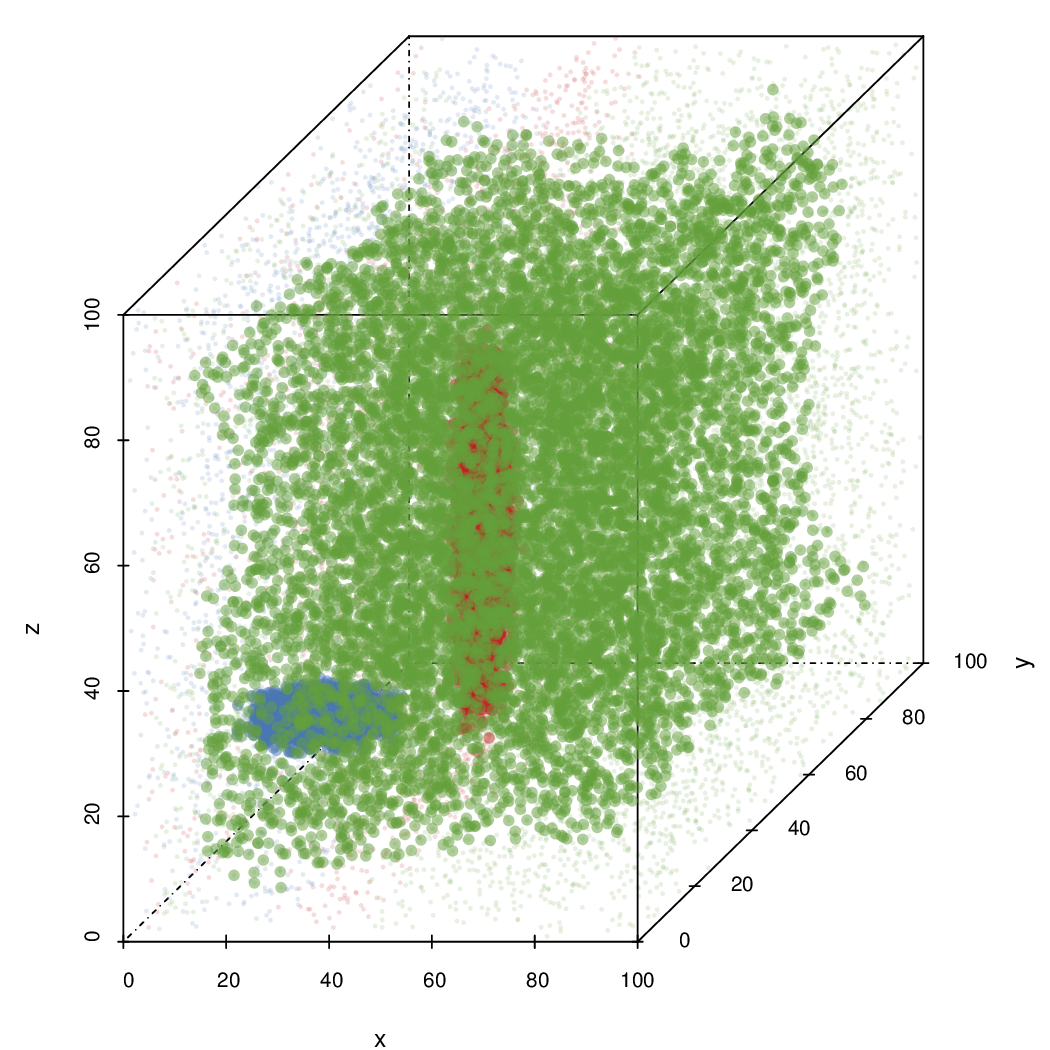
\includegraphics[keepaspectratio=true, width=\textwidth, height=0.23\textheight]{discussion/img/baakman_2_abs_error_mbeSmallerThansambe.pdf}
			\caption{Dataset \baakmanTwo}
			\label{fig:discussion:multisphere:mbeLowerError:baakman2}
		\end{subfigure}	
		\caption{Low opacity scatter plot of dataset \subref{fig:discussion:multisphere:mbeLowerError:ferdosi2} \ferdosiTwo and \subref{fig:discussion:multisphere:mbeLowerError:baakman2} \baakmanTwo with an overlay of high opacity larger points where the absolute error of \mbe is smaller than the absolute error of \sambe.}
		\label{fig:discussion:multisphere:two:mbeLowerError}
	\end{figure}

	% Ferdosi 3 & Baakman 3
	Plotting the densities estimated by \sambe versus the densities estimated by \mbe in \cref{fig:discussion:multisphere:four:mbevssambe} shows that the differences between the estimators are as small as indicated by the \mse for nearly all points, \sambe slightly underestimates points drawn from the noise that has a high density. As the noise component by itself has an uniform density these points noise points are quite likely positioned near the center of one of the Gaussian components. \Cref{fig:discussion:multisphere:four:mbeLowerError} shows that the shape-adaptive estimator outperforms the symmetric estimator consistently on points near the boundary of the dataset. Although it is not visible due to occlusion in \cref{fig:discussion:multisphere:mbeLowerError:ferdosi3,fig:discussion:multisphere:mbeLowerError:baakman3} approximately half of the points in the center have a lower absolute error for \sambe than for \mbe. Taking a closer look at the Gaussians we find a correlation between which estimator has the lowest absolute error on a point and the distance of that point to the mean. For dataset \ferdosiThree we can say that \sambe performs better on points farther away from the mean, whereas \mbe is better in approximating the density of points nearer to the mean of a distribution. In \baakmanThree this effect is even stronger. 

	% Difference between ferdosi 2 and three
	Interestingly the shape defined by the points where the absolute error of \mbe is lower than that of \sambe defines a square in the dataset with two Gaussian components and approximately a sphere in the dataset with four Gaussian components. We expect that this difference is caused by the Gaussian components that are nearer to the boundaries in dataset \ferdosiThree and \baakmanThree. 

	\begin{figure}
		\centering
		\begin{subfigure}{0.23\textwidth}
			\centering
			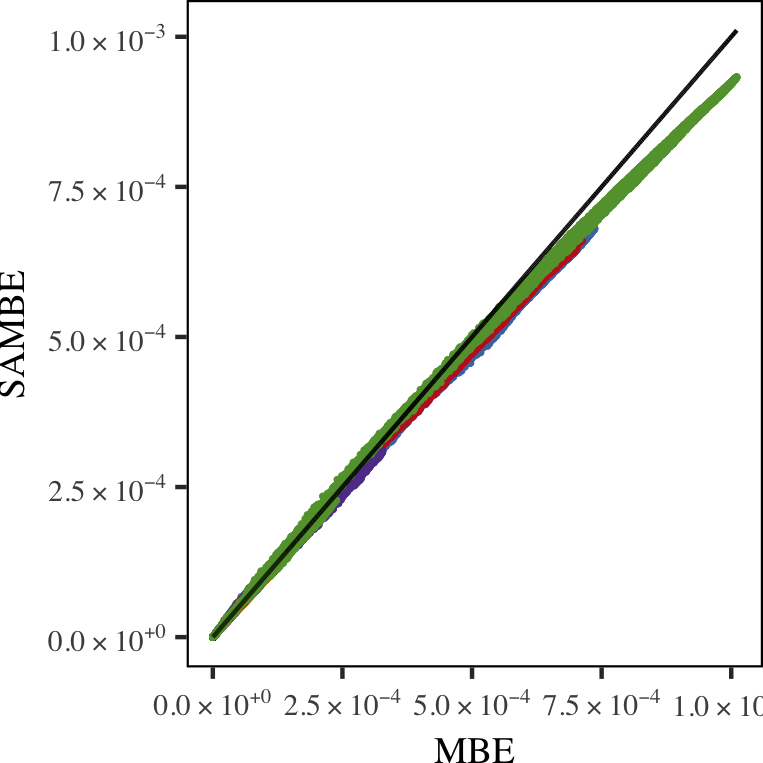
\includegraphics[keepaspectratio=true, width=\textwidth, height=0.23\textheight]{discussion/img/ferdosi_3_120000_mbe_sambe.png}
			\caption{Dataset \ferdosiThree}
			\label{fig:discussion:multisphere:mbevssambe:ferdosi3}
		\end{subfigure}
		\begin{subfigure}{0.23\textwidth}
			\centering
			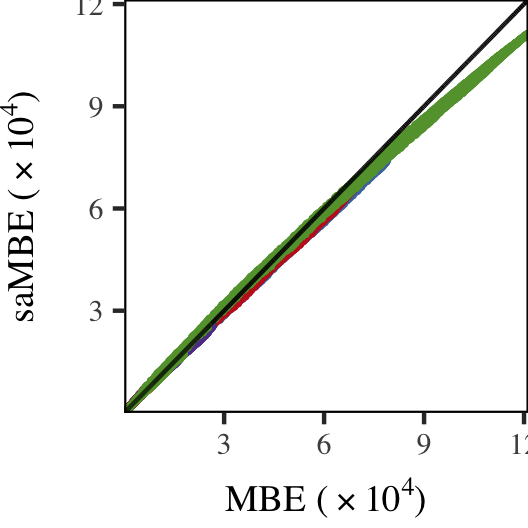
\includegraphics[keepaspectratio=true, width=\textwidth, height=0.23\textheight]{discussion/img/baakman_3_120000_mbe_sambe.png}
			\caption{Dataset \baakmanThree}
			\label{fig:discussion:multisphere:mbevssambe:baakman3}
		\end{subfigure}	
		\caption{Plots of the density estimated by \sambe as a function of those estimated by \mbe for dataset %
			\subref{fig:discussion:multisphere:mbevssambe:ferdosi3} % 
			\ferdosiTwo and %
			\subref{fig:discussion:multisphere:mbevssambe:baakman3} %
			\baakmanTwo.
		}
		\label{fig:discussion:multisphere:four:mbevssambe}
	\end{figure}

	\begin{figure}
		\centering
		\begin{subfigure}{0.23\textwidth}
			\centering
			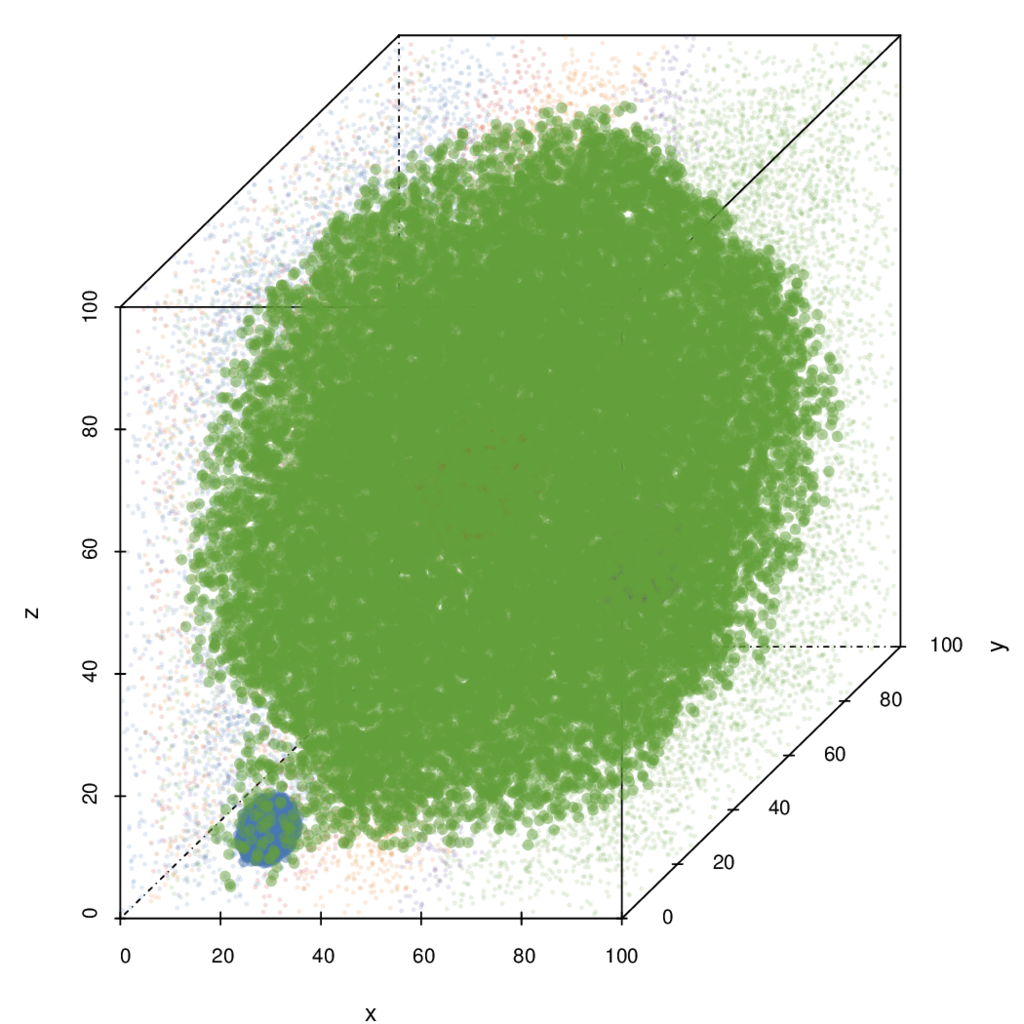
\includegraphics[keepaspectratio=true, width=\textwidth, height=0.23\textheight]{discussion/img/ferdosi_3_abs_error_mbeSmallerThansambe.pdf}
			\caption{Dataset \ferdosiThree}
			\label{fig:discussion:multisphere:mbeLowerError:ferdosi3}
		\end{subfigure}
		\begin{subfigure}{0.23\textwidth}
			\centering
			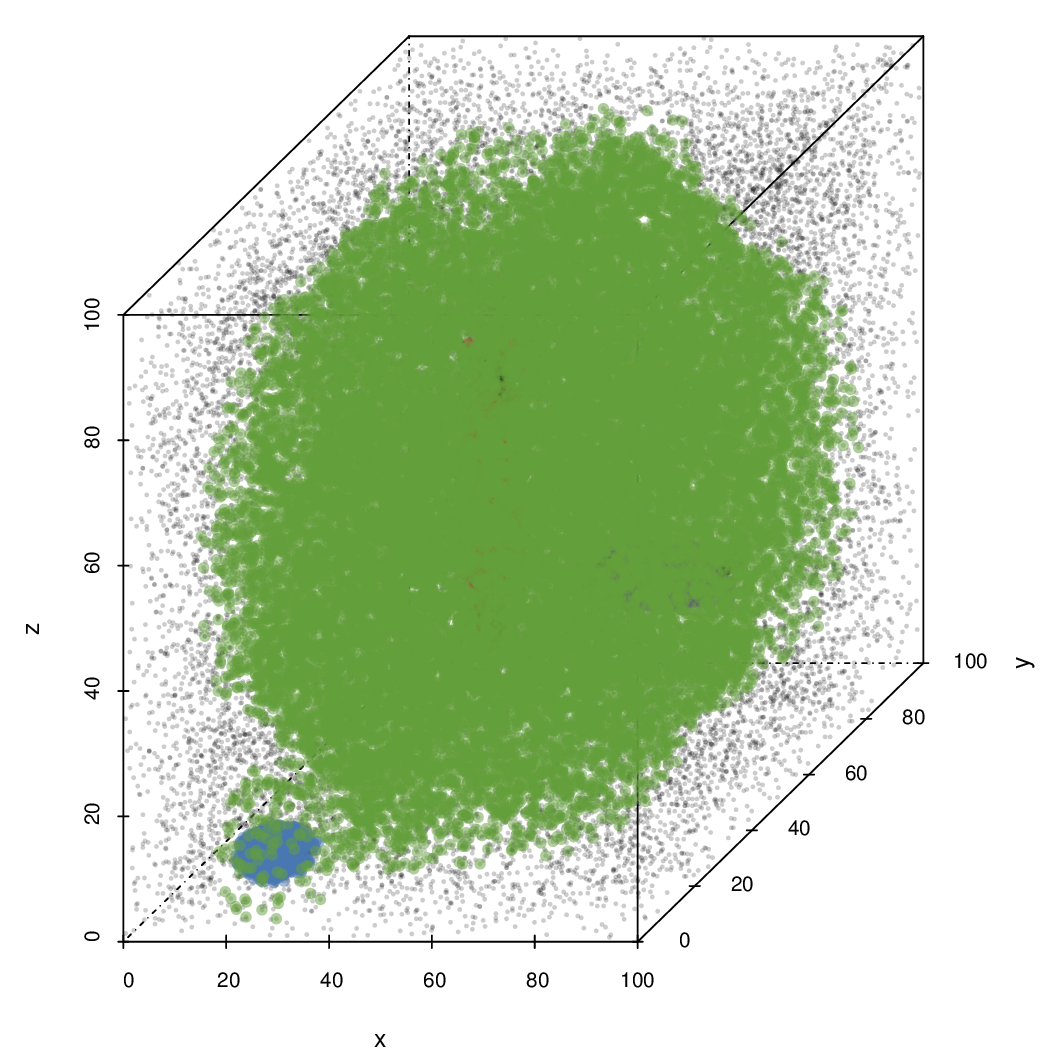
\includegraphics[keepaspectratio=true, width=\textwidth, height=0.23\textheight]{discussion/img/baakman_3_abs_error_mbeSmallerThansambe.pdf}
			\caption{Dataset \baakmanThree}
			\label{fig:discussion:multisphere:mbeLowerError:baakman3}
		\end{subfigure}	
		\caption{Low opacity scatter plot of dataset 			\subref{fig:discussion:multisphere:mbeLowerError:ferdosi3} % 
			\ferdosiTwo and \subref{fig:discussion:multisphere:mbeLowerError:baakman3} \baakmanTwo with the points where the absolute error of \mbe is smaller than the absolute error of \sambe emphasized.
		}
		\label{fig:discussion:multisphere:four:mbeLowerError}
	\end{figure}	